\section{Welfare and policy}

\subsection{Welfare framework}
The firm's choice $b^*$ is privately optimal but socially inefficient. A social planner's objective function, $SWF(b) = V(b) - E(b)$, must include the external costs $E(b)$ of bias. These costs are many. First, there are Distributional Costs, as the bias `$b$` directly harms the disadvantaged group ($g=1$) by lowering their probability of being hired for any given level of productivity $\theta$, creating an equity-efficiency trade-off from the planner's perspective. Second, there are Dynamic Costs, as persistent bias can discourage human capital investment by the disadvantaged group, potentially creating a self-fulfilling prophecy where ex-ante identical groups become ex-post different \citep{Coate1993}, and can also erode social trust and political stability. Finally, there is Allocative Inefficiency, because while the firm optimizes its own hiring decisions, the bias across multiple firms may lead to suboptimal allocation of talent across the economy.
The social optimum $b^{**}$ that maximizes $SWF(b)$ will be strictly less than $b^*$, creating a deadweight loss and justifying policy intervention.

\subsection{Policy instruments}

Our analysis suggests that prescriptive regulations, such as a simple mandate forcing firms to set bias to zero ($b=0$), are inefficient. Such policies bluntly override the firm's optimization without addressing the underlying technological trade-off, potentially sacrificing significant predictive accuracy for fairness. A more effective approach, visualized in Figure \ref{fig:policy}, is to employ incentive-based instruments that reshape the firm's objective function to better align private and social goals.

\paragraph{R\&D subsidies to improve the technological frontier.}
The most efficient intervention is one that targets the root cause of the problem: the severity of the fairness-accuracy trade-off itself. Policies that subsidize research and development can incentivize the creation of new algorithms that lower the technology coupling parameter, $\kappa$. A lower $\kappa$ makes the firm's value function flatter, as formally established in Lemma 4 in the Appendix. As illustrated by the green curve in Figure \ref{fig:policy}, this reduction in the curvature of the profit function diminishes the marginal return to bias, causing the firm's optimal choice to decrease significantly from the baseline $b^*$.

\paragraph{Pigouvian taxation to internalize externalities.}
A second approach is to accept the technological frontier as given but force the firm to account for the social costs of its decision. A regulator could impose a Pigouvian tax, $\tau$, for each unit of bias, which alters the firm's problem to $\max_b V(b) - \tau b$. This compels the firm to internalize the negative externality described by the cost function $E(b)$. Figure \ref{fig:policy} demonstrates this effect powerfully: the red curve, representing the firm's payoff under taxation, is shifted downward and tilted, moving the optimum dramatically leftward to a level of bias near the social optimum $b^{**}$. As derived in Appendix A.5, an optimally chosen tax, $\tau^*$, can induce the firm to select the socially optimal level of bias.

\paragraph{Transparency mandates to leverage market forces.}
Finally, policy can leverage market mechanisms to create endogenous costs for bias. Mandates requiring firms to disclose the fairness properties and trade-offs of their algorithms would not prescribe a specific choice. Instead, they would empower stakeholders (for example, potential employees, customers, or investors) to react to a firm's level of bias. This would effectively endogenize the external cost function $E(b)$ through reputational damage and competitive pressure.

\begin{figure}[H]
    \centering
    % The path is relative from the 'sections' folder up to the project root, then down to 'figures'
    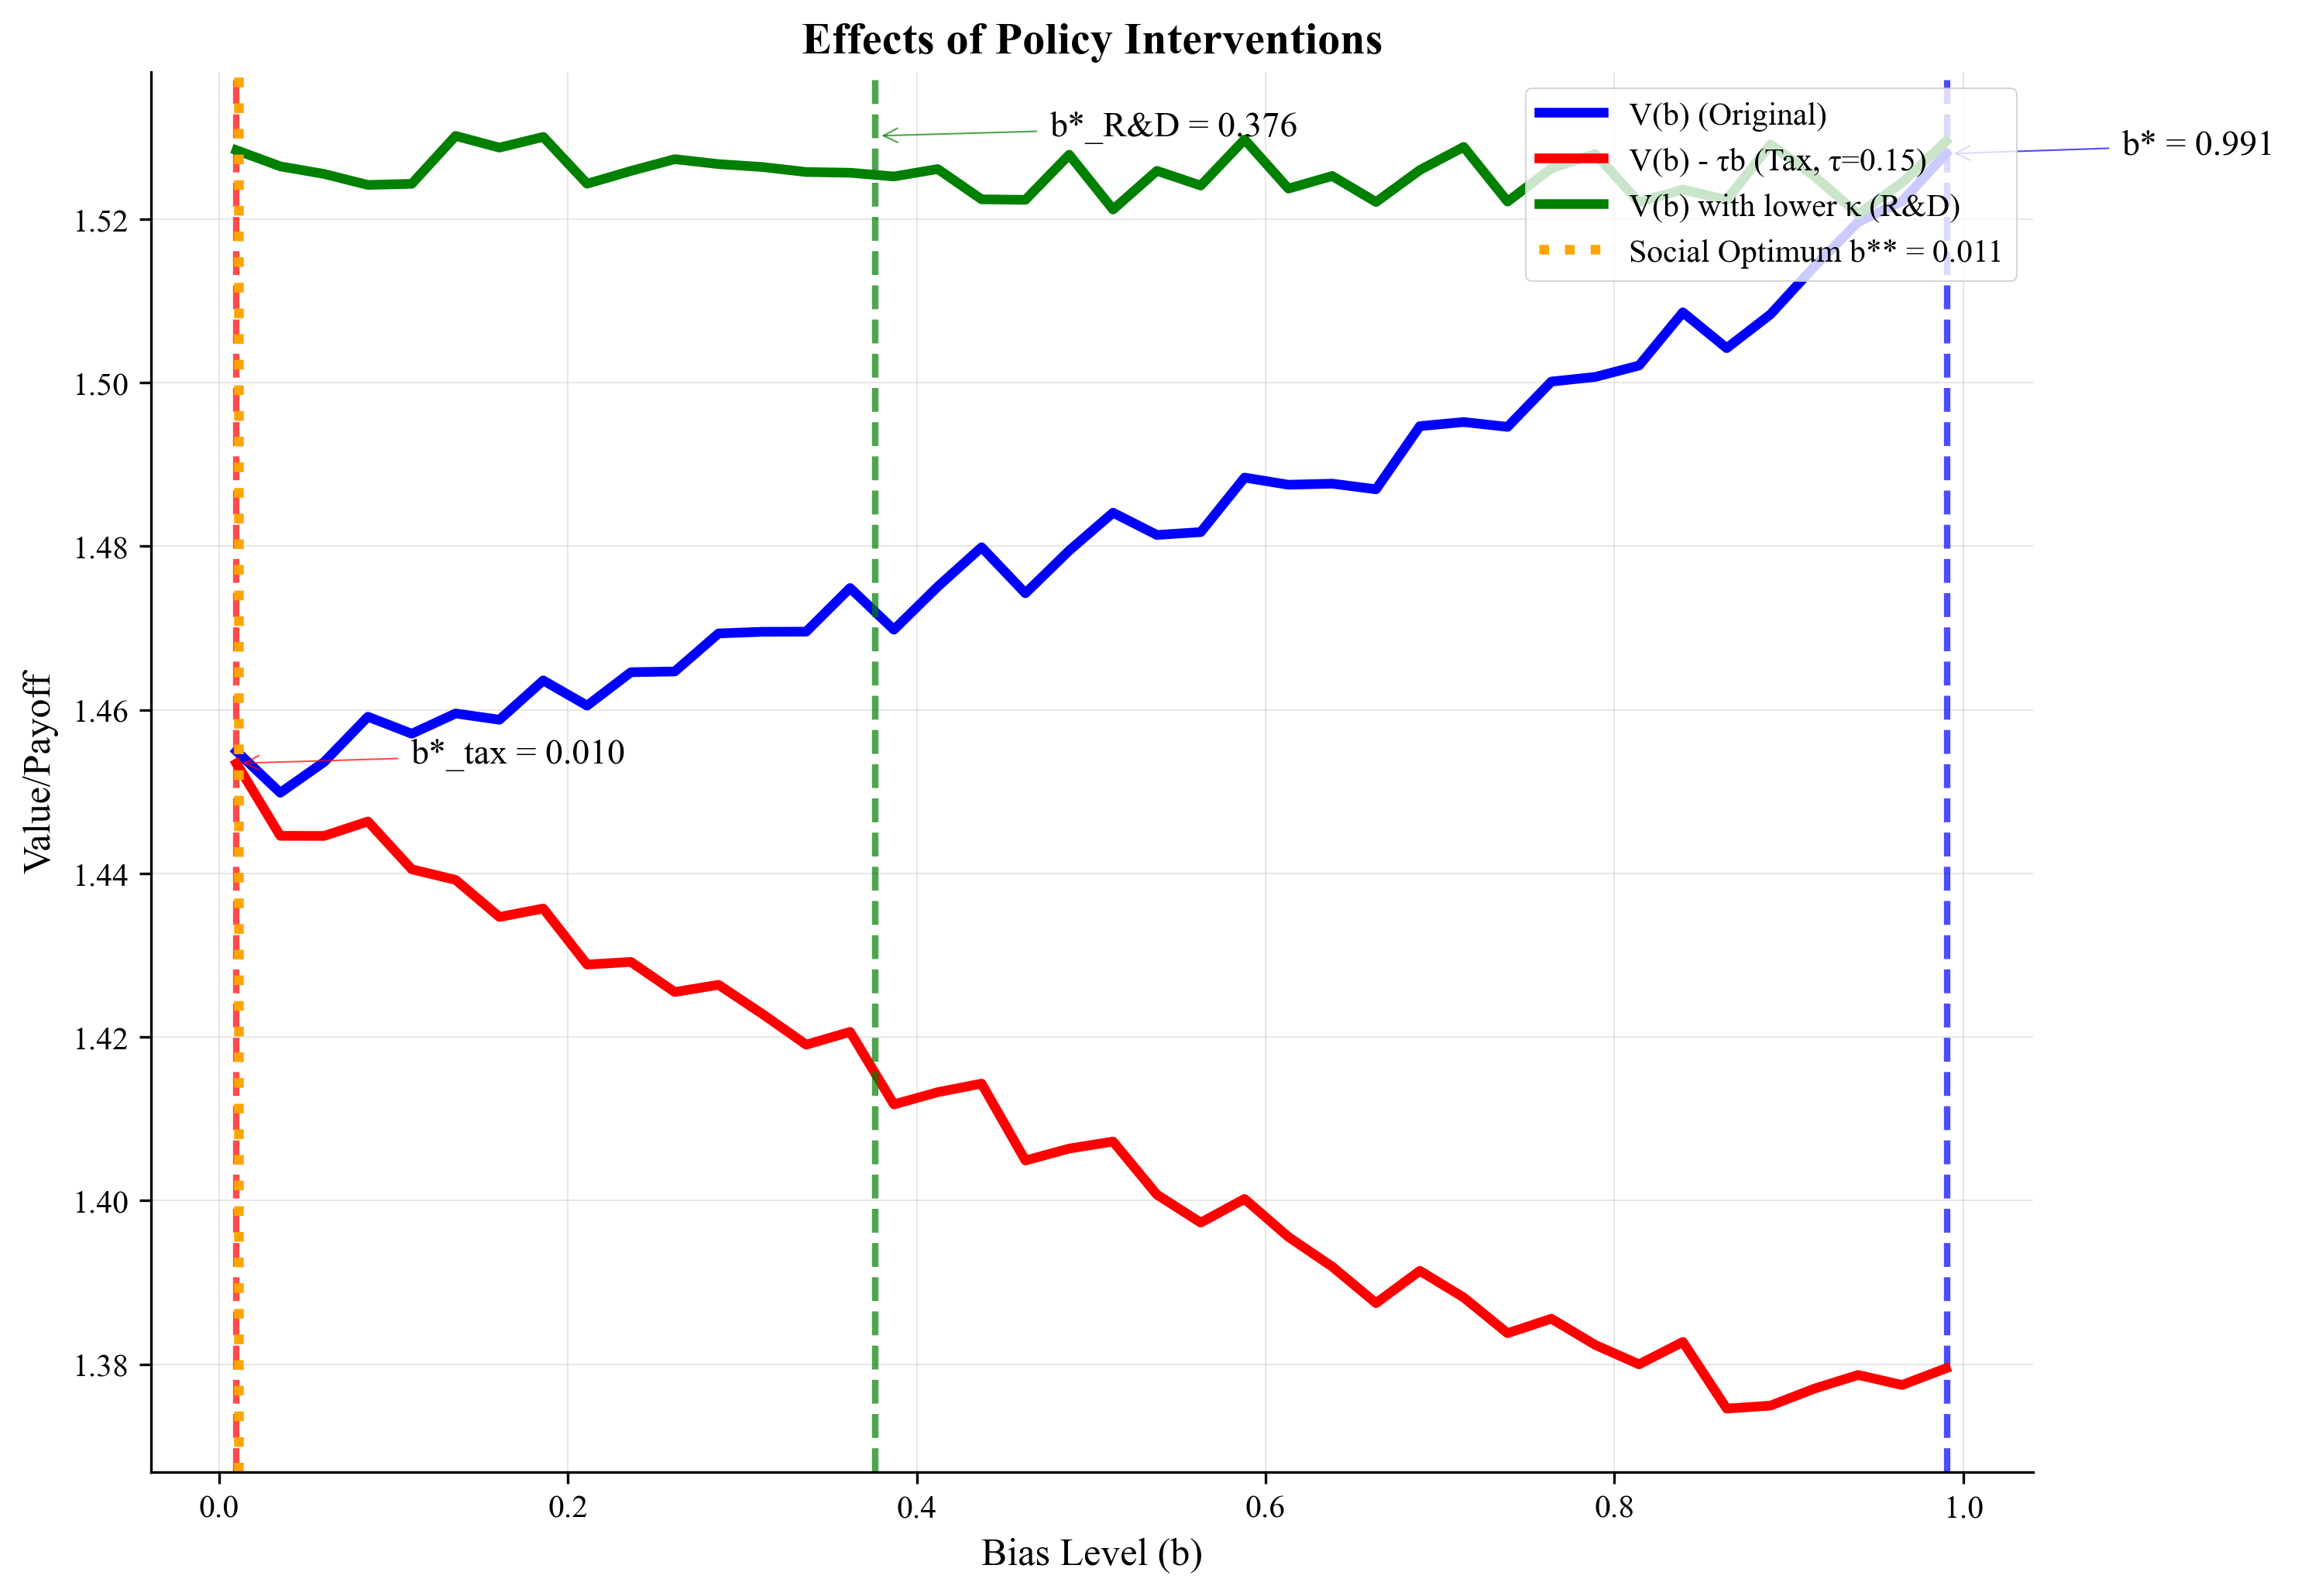
\includegraphics[width=1\textwidth]{../figures/figure_2_policy_interventions.png}
    \caption[Effects of policy interventions]{\textbf{Effects of policy interventions.} The baseline value function (blue) is maximized at a high private optimum, $b^*=0.991$. An R\&D subsidy that lowers $\kappa$ flattens the value function (green), reducing the optimal bias to $b^*_{\text{R\&D}}=0.376$. A Pigouvian tax (red) makes high levels of bias unprofitable, shifting the optimum to $b^*_{\text{tax}}=0.010$, which is close to the social optimum $b^{**}=0.011$ (orange).}
    \label{fig:policy}
\end{figure}